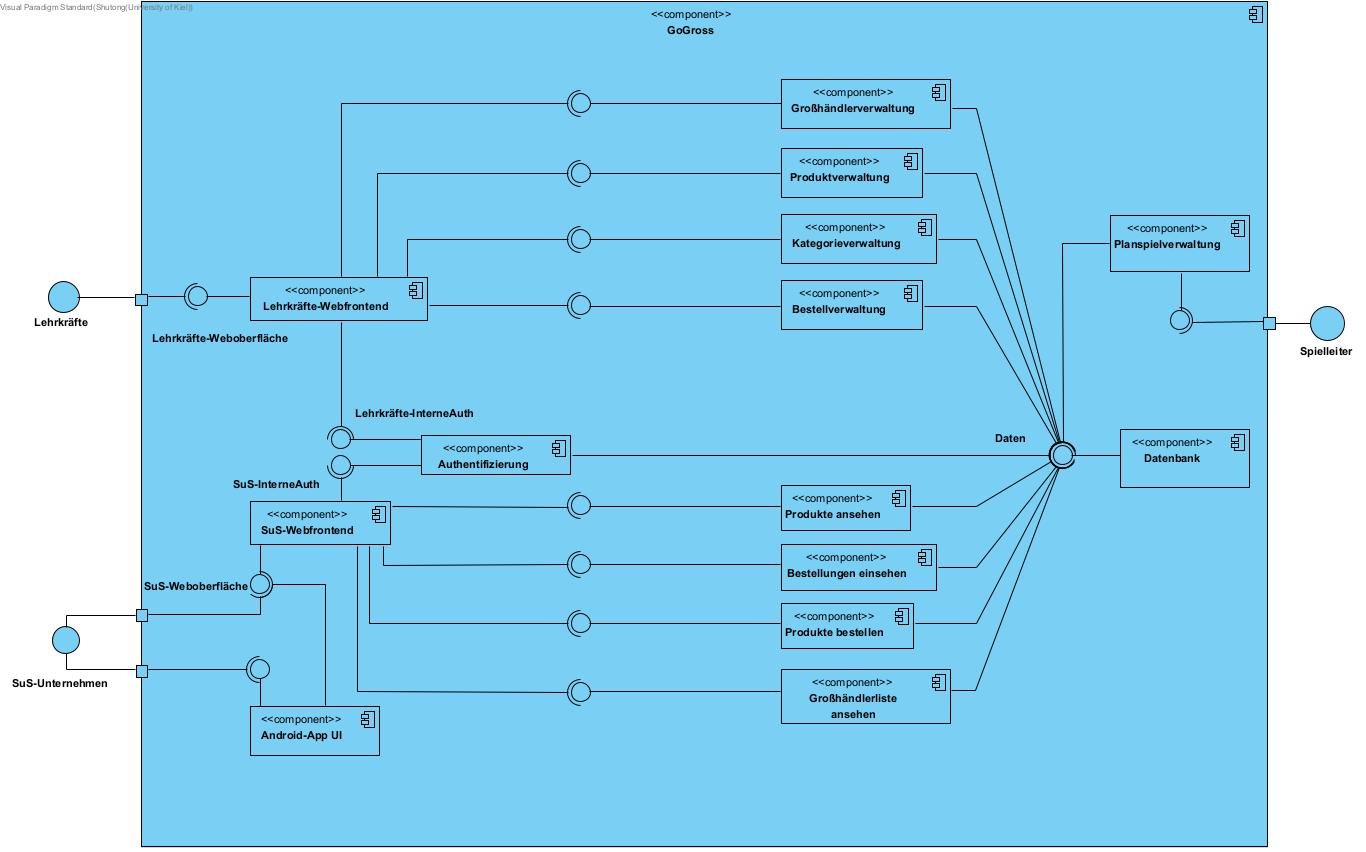
\includegraphics[width=\textwidth]{img/Component}
\label{fig: GoGross Komponentendiagramm}

\begin{itemize}
    \item Der Spielleiter kann alle Planspiele über die Kommandozeile verwalten. Die Verwaltung umfasst die Erstellung, das Beenden sowie den Import und Export von Spielständen.
    \item Die Lehrkräfte nutzen eine über HTTPS gesicherte Weboberfläche, die über eine Authentifizierungskomponente gesichert ist. Nach erfolgreicher Authentifizierung können diese auf verschiedene Verwaltungskomponenten zugreifen. Diese ermöglichen das Management von Großhändlern, Produkten, Kategorien und Bestellungen. Wie zum Beispiel das Löschen, Hinzufügen, Importieren oder Exportieren.
\newpage
    \item SuS-Unternehmen verwenden entweder eine Weboberfläche oder eine auf der Weboberfläche basierende Android-Anwendung, um sich zu authentifizieren und anschließend Zugriff auf verschiedene Bestellkomponenten zu erhalten. So können diese Großhändler, Produkte und Bestellungen ansehen sowie Bestellungen tätigen. 
    \item Die Authentifizierungskomponente gewährleistet einen sicheren Zugang für Lehrkräfte und SuS-Unternehmen. Diese reguliert den Zugriff mithilfe der gespeicherten Benutzerdaten in der Datenbank und sichert somit die Integrität sowie Sicherheit des Systems.
    \item Das GoGross System wird von einer internen Datenbankkomponente gestützt, welche relevante Informationen und Beziehungen speichert. Diese Datenbank wird von den verschiedenen Komponenten zur Ausführung ihrer spezifischen Aufgaben abgefragt und verändert. 
\end{itemize}